%-------------------------------------------------------------------------------
%	RoboCell PRESENTATION SLIDES
%-------------------------------------------------------------------------------
\section{RoboCell}
\begin{frame}
  RoboCell:\\
  New micro-world basement for the robotics
\end{frame}

%------------------------------------------------
\subsection{The problem} % Sections can be created in order to organize your presentation into discrete blocks, all sections and subsections are automatically printed in the table of contents as an overview of the talk
%------------------------------------------------
\begin{frame}
\frametitle{Macro robotic system problems}
\begin{columns}[c] % The "c" option specifies centered vertical alignment while the "t" option is used for top vertical alignment

\column{.45\textwidth} % Left column and width
\begin{itemize}
\item \textbf{Homeostasis} - the super-stability via impact over environment 
\item \textbf{Reproduction} -self replication, regeneration
\item \textbf{Feeding}
\item \textbf{Specialization}
\item \textbf{Self organisation/self-assembly}
\item \textbf{Balance}
\item \textbf{Randomness} - for example the Brownian motion
\end{itemize}

\column{.6\textwidth} % Right column and width
%------------------------------------------------
\begin{figure}
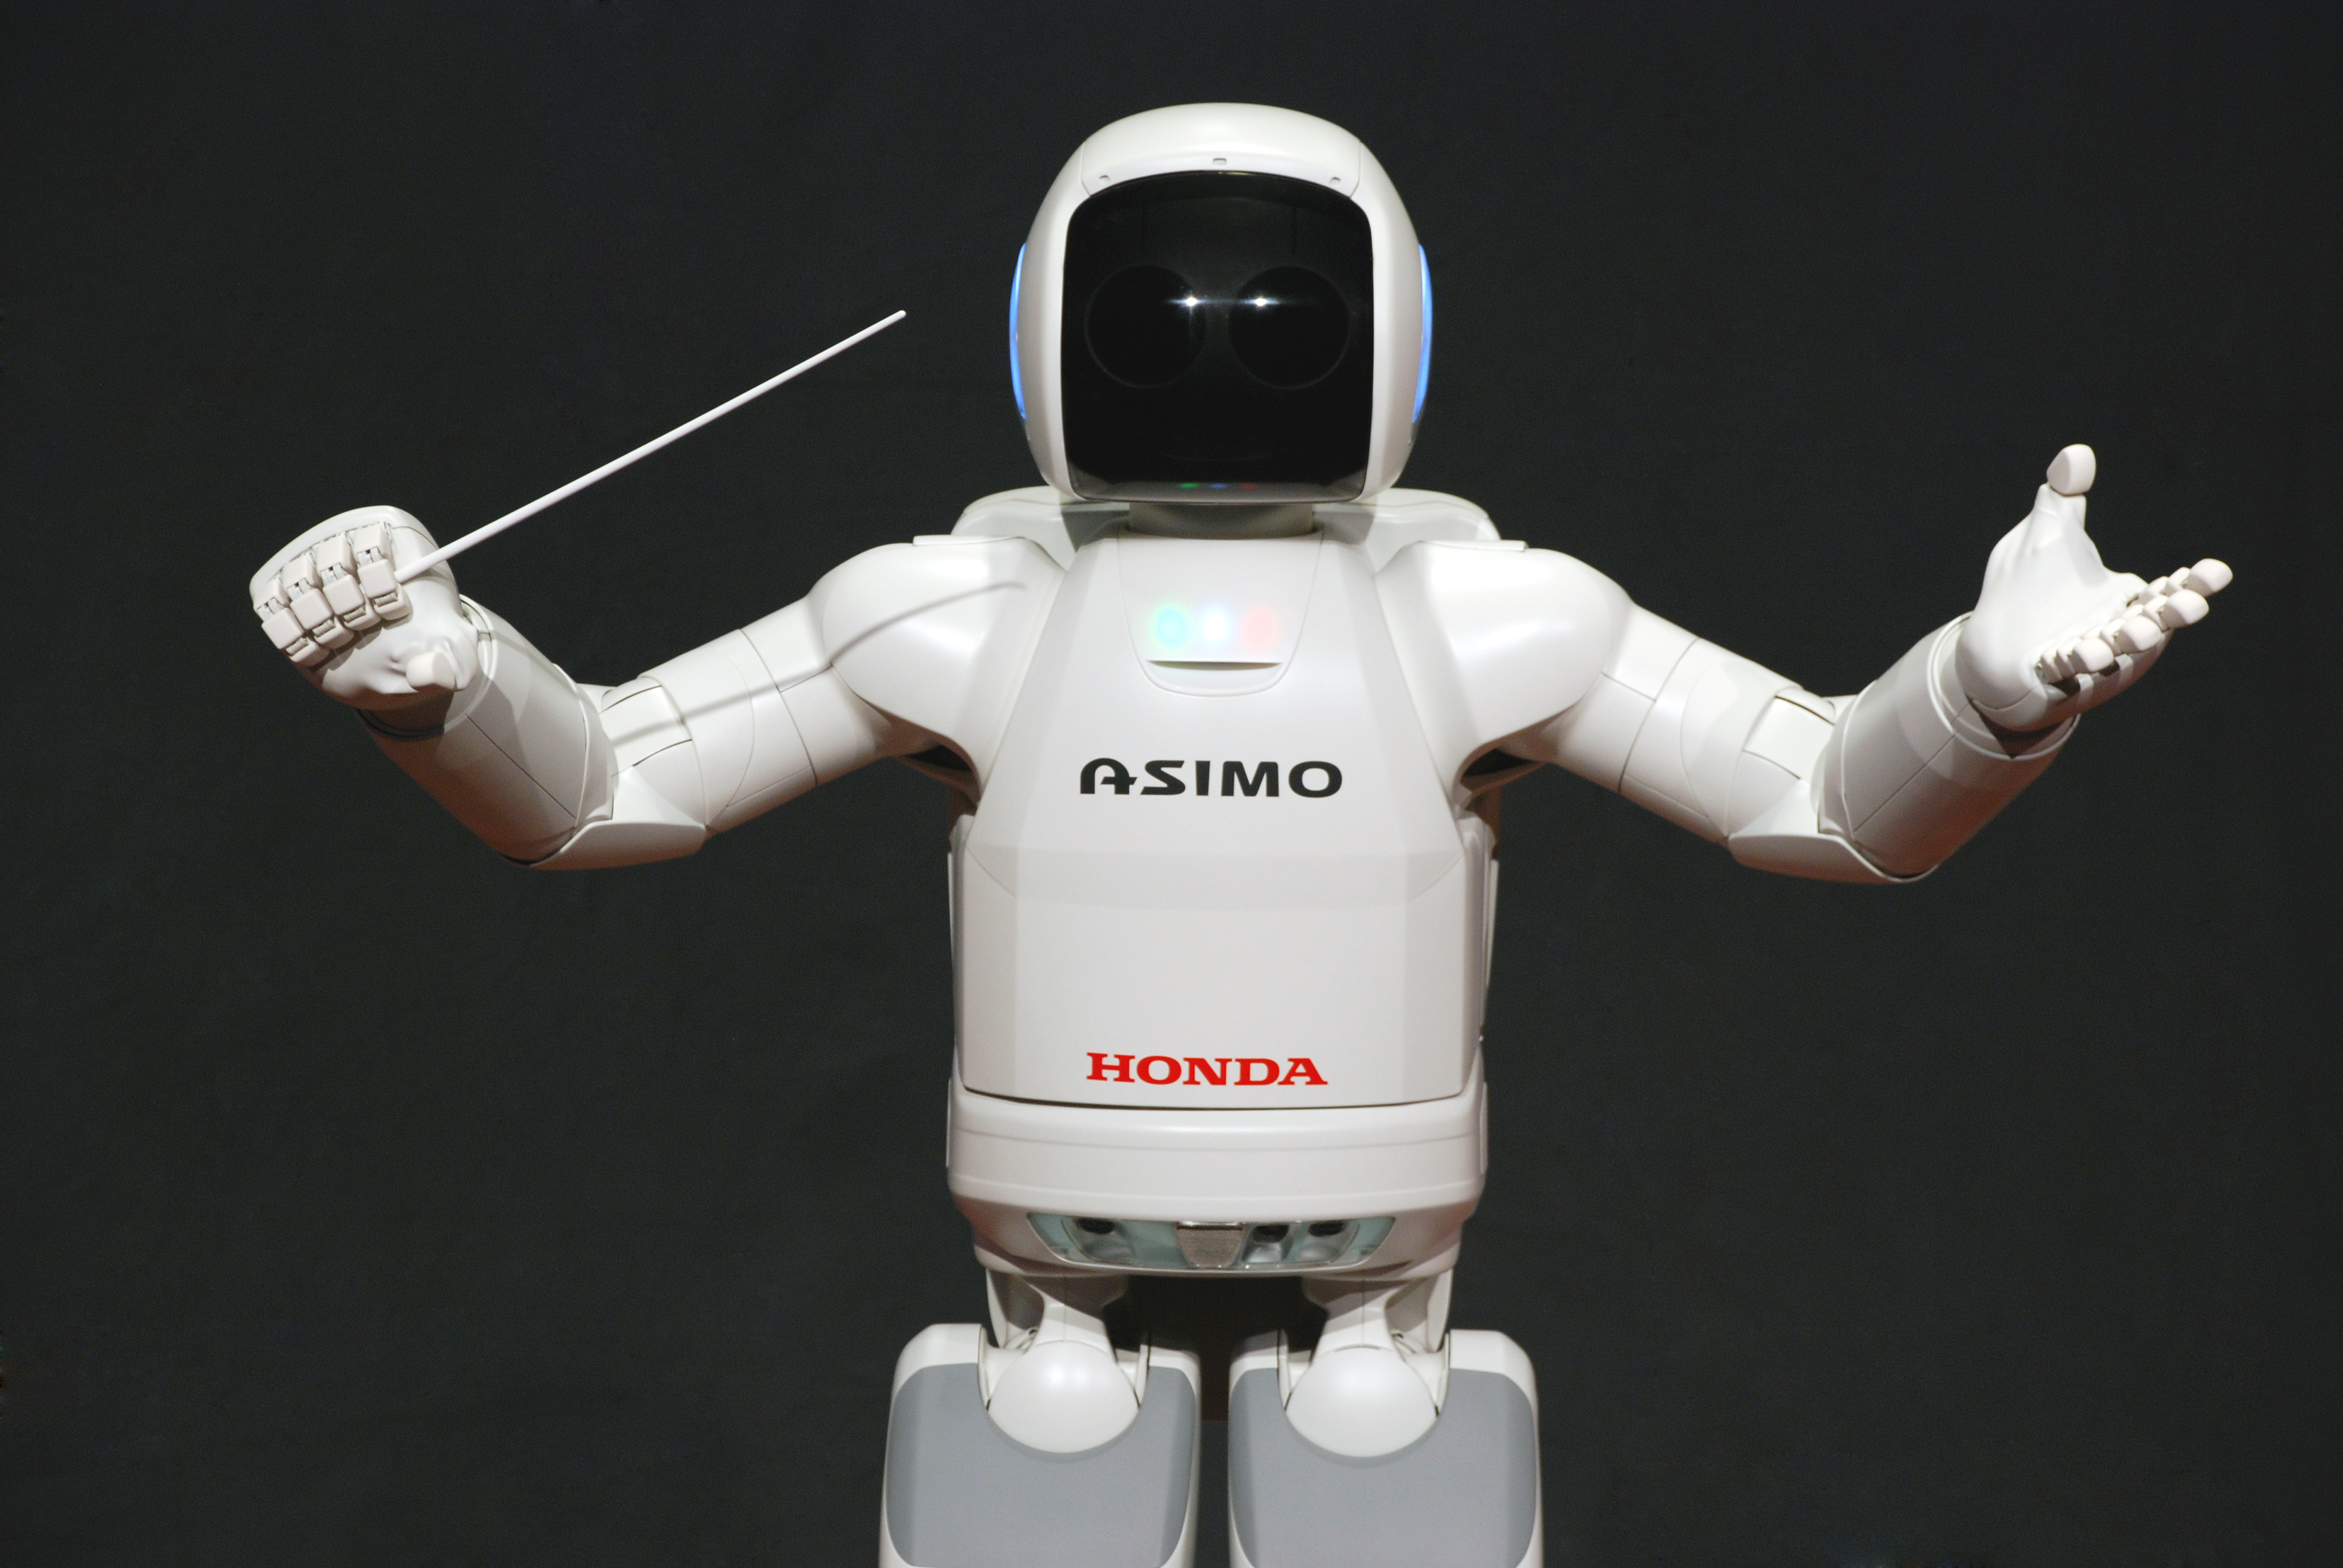
\includegraphics[width=1.0\linewidth]{ASIMO_Conducting}
\end{figure}
%------------------------------------------------
\end{columns}
\end{frame}

%------------------------------------------------
\subsection{Questions}
%------------------------------------------------
\begin{frame}
\frametitle{Questions}

Primary:
\begin{itemize}
\item Can we create cell of different nature (non organic)?
\item Can we create organ of different nature ?
\item Can we integrate organs done with cells of different nature?
\item Can we update properties of cell by design?
\end{itemize}

Derivatives:
\begin{itemize}
\item Use radio frequency to communicate
\item  Can we create cells sensitive to radio frequency ?
\item  Can we make cell doing digital calculations ?
\item  Can we create organism to exist in vacuum?
\item  Can we make artificial organism faster stronger?
\end{itemize}
\end{frame}
%------------------------------------------------

%------------------------------------------------
\subsection{Solution}
%------------------------------------------------
\begin{frame}
\frametitle{Solution}

\begin{itemize}
\item Simulation of cell structures
\item Computational experiments with new nature of cell and cellular mechanisms
\item Self replication with silicon cells
\item Cells with conductivity and digital computation capacity
\end{itemize}

\end{frame}
%------------------------------------------------
